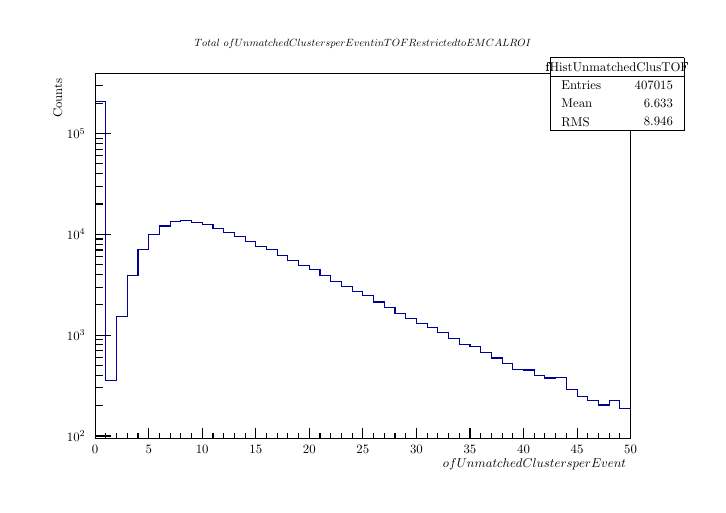
\begin{tikzpicture}
\pgfdeclareplotmark{cross} {
\pgfpathmoveto{\pgfpoint{-0.3\pgfplotmarksize}{\pgfplotmarksize}}
\pgfpathlineto{\pgfpoint{+0.3\pgfplotmarksize}{\pgfplotmarksize}}
\pgfpathlineto{\pgfpoint{+0.3\pgfplotmarksize}{0.3\pgfplotmarksize}}
\pgfpathlineto{\pgfpoint{+1\pgfplotmarksize}{0.3\pgfplotmarksize}}
\pgfpathlineto{\pgfpoint{+1\pgfplotmarksize}{-0.3\pgfplotmarksize}}
\pgfpathlineto{\pgfpoint{+0.3\pgfplotmarksize}{-0.3\pgfplotmarksize}}
\pgfpathlineto{\pgfpoint{+0.3\pgfplotmarksize}{-1.\pgfplotmarksize}}
\pgfpathlineto{\pgfpoint{-0.3\pgfplotmarksize}{-1.\pgfplotmarksize}}
\pgfpathlineto{\pgfpoint{-0.3\pgfplotmarksize}{-0.3\pgfplotmarksize}}
\pgfpathlineto{\pgfpoint{-1.\pgfplotmarksize}{-0.3\pgfplotmarksize}}
\pgfpathlineto{\pgfpoint{-1.\pgfplotmarksize}{0.3\pgfplotmarksize}}
\pgfpathlineto{\pgfpoint{-0.3\pgfplotmarksize}{0.3\pgfplotmarksize}}
\pgfpathclose
\pgfusepathqstroke
}
\pgfdeclareplotmark{cross*} {
\pgfpathmoveto{\pgfpoint{-0.3\pgfplotmarksize}{\pgfplotmarksize}}
\pgfpathlineto{\pgfpoint{+0.3\pgfplotmarksize}{\pgfplotmarksize}}
\pgfpathlineto{\pgfpoint{+0.3\pgfplotmarksize}{0.3\pgfplotmarksize}}
\pgfpathlineto{\pgfpoint{+1\pgfplotmarksize}{0.3\pgfplotmarksize}}
\pgfpathlineto{\pgfpoint{+1\pgfplotmarksize}{-0.3\pgfplotmarksize}}
\pgfpathlineto{\pgfpoint{+0.3\pgfplotmarksize}{-0.3\pgfplotmarksize}}
\pgfpathlineto{\pgfpoint{+0.3\pgfplotmarksize}{-1.\pgfplotmarksize}}
\pgfpathlineto{\pgfpoint{-0.3\pgfplotmarksize}{-1.\pgfplotmarksize}}
\pgfpathlineto{\pgfpoint{-0.3\pgfplotmarksize}{-0.3\pgfplotmarksize}}
\pgfpathlineto{\pgfpoint{-1.\pgfplotmarksize}{-0.3\pgfplotmarksize}}
\pgfpathlineto{\pgfpoint{-1.\pgfplotmarksize}{0.3\pgfplotmarksize}}
\pgfpathlineto{\pgfpoint{-0.3\pgfplotmarksize}{0.3\pgfplotmarksize}}
\pgfpathclose
\pgfusepathqfillstroke
}
\pgfdeclareplotmark{newstar} {
\pgfpathmoveto{\pgfqpoint{0pt}{\pgfplotmarksize}}
\pgfpathlineto{\pgfqpointpolar{44}{0.5\pgfplotmarksize}}
\pgfpathlineto{\pgfqpointpolar{18}{\pgfplotmarksize}}
\pgfpathlineto{\pgfqpointpolar{-20}{0.5\pgfplotmarksize}}
\pgfpathlineto{\pgfqpointpolar{-54}{\pgfplotmarksize}}
\pgfpathlineto{\pgfqpointpolar{-90}{0.5\pgfplotmarksize}}
\pgfpathlineto{\pgfqpointpolar{234}{\pgfplotmarksize}}
\pgfpathlineto{\pgfqpointpolar{198}{0.5\pgfplotmarksize}}
\pgfpathlineto{\pgfqpointpolar{162}{\pgfplotmarksize}}
\pgfpathlineto{\pgfqpointpolar{134}{0.5\pgfplotmarksize}}
\pgfpathclose
\pgfusepathqstroke
}
\pgfdeclareplotmark{newstar*} {
\pgfpathmoveto{\pgfqpoint{0pt}{\pgfplotmarksize}}
\pgfpathlineto{\pgfqpointpolar{44}{0.5\pgfplotmarksize}}
\pgfpathlineto{\pgfqpointpolar{18}{\pgfplotmarksize}}
\pgfpathlineto{\pgfqpointpolar{-20}{0.5\pgfplotmarksize}}
\pgfpathlineto{\pgfqpointpolar{-54}{\pgfplotmarksize}}
\pgfpathlineto{\pgfqpointpolar{-90}{0.5\pgfplotmarksize}}
\pgfpathlineto{\pgfqpointpolar{234}{\pgfplotmarksize}}
\pgfpathlineto{\pgfqpointpolar{198}{0.5\pgfplotmarksize}}
\pgfpathlineto{\pgfqpointpolar{162}{\pgfplotmarksize}}
\pgfpathlineto{\pgfqpointpolar{134}{0.5\pgfplotmarksize}}
\pgfpathclose
\pgfusepathqfillstroke
}
\definecolor{c}{rgb}{1,1,1};
\draw [color=c, fill=c] (0,0) rectangle (8.5,5.78879);
\draw [color=c, fill=c] (0.85,0.578879) rectangle (7.65,5.20991);
\definecolor{c}{rgb}{0,0,0};
\draw [c] (0.85,0.578879) -- (0.85,5.20991) -- (7.65,5.20991) -- (7.65,0.578879) -- (0.85,0.578879);
\definecolor{c}{rgb}{1,1,1};
\draw [color=c, fill=c] (0.85,0.578879) rectangle (7.65,5.20991);
\definecolor{c}{rgb}{0,0,0};
\draw [c] (0.85,0.578879) -- (0.85,5.20991) -- (7.65,5.20991) -- (7.65,0.578879) -- (0.85,0.578879);
\definecolor{c}{rgb}{0,0,0.6};
\draw [c] (0.85,4.85459) -- (0.986,4.85459) -- (0.986,1.31474) -- (1.122,1.31474) -- (1.122,2.12224) -- (1.258,2.12224) -- (1.258,2.64408) -- (1.394,2.64408) -- (1.394,2.98048) -- (1.53,2.98048) -- (1.53,3.17468) -- (1.666,3.17468) -- (1.666,3.27636)
 -- (1.802,3.27636) -- (1.802,3.33272) -- (1.938,3.33272) -- (1.938,3.34484) -- (2.074,3.34484) -- (2.074,3.32215) -- (2.21,3.32215) -- (2.21,3.29445) -- (2.346,3.29445) -- (2.346,3.24262) -- (2.482,3.24262) -- (2.482,3.19153) -- (2.618,3.19153) --
 (2.618,3.14076) -- (2.754,3.14076) -- (2.754,3.08358) -- (2.89,3.08358) -- (2.89,3.02042) -- (3.026,3.02042) -- (3.026,2.976) -- (3.162,2.976) -- (3.162,2.90702) -- (3.298,2.90702) -- (3.298,2.84168) -- (3.434,2.84168) -- (3.434,2.77231) --
 (3.57,2.77231) -- (3.57,2.72468) -- (3.706,2.72468) -- (3.706,2.65318) -- (3.842,2.65318) -- (3.842,2.57469) -- (3.978,2.57469) -- (3.978,2.50541) -- (4.114,2.50541) -- (4.114,2.44585) -- (4.25,2.44585) -- (4.25,2.3926) -- (4.386,2.3926) --
 (4.386,2.31197) -- (4.522,2.31197) -- (4.522,2.24681) -- (4.658,2.24681) -- (4.658,2.16456) -- (4.794,2.16456) -- (4.794,2.10246) -- (4.93,2.10246) -- (4.93,2.04024) -- (5.066,2.04024) -- (5.066,1.98725) -- (5.202,1.98725) -- (5.202,1.92346) --
 (5.338,1.92346) -- (5.338,1.85138) -- (5.474,1.85138) -- (5.474,1.77132) -- (5.61,1.77132) -- (5.61,1.7416) -- (5.746,1.7416) -- (5.746,1.67611) -- (5.882,1.67611) -- (5.882,1.60094) -- (6.018,1.60094) -- (6.018,1.53334) -- (6.154,1.53334) --
 (6.154,1.45638) -- (6.29,1.45638) -- (6.29,1.44781) -- (6.426,1.44781) -- (6.426,1.3741) -- (6.562,1.3741) -- (6.562,1.34669) -- (6.698,1.34669) -- (6.698,1.35695) -- (6.834,1.35695) -- (6.834,1.20038) -- (6.97,1.20038) -- (6.97,1.11531) --
 (7.106,1.11531) -- (7.106,1.0612) -- (7.242,1.0612) -- (7.242,1.00399) -- (7.378,1.00399) -- (7.378,1.0612) -- (7.514,1.0612) -- (7.514,0.96426) -- (7.65,0.96426);
\definecolor{c}{rgb}{1,1,1};
\draw [color=c, fill=c] (6.63,4.48631) rectangle (8.33,5.41252);
\definecolor{c}{rgb}{0,0,0};
\draw [c] (6.63,4.48631) -- (8.33,4.48631);
\draw [c] (8.33,4.48631) -- (8.33,5.41252);
\draw [c] (8.33,5.41252) -- (6.63,5.41252);
\draw [c] (6.63,5.41252) -- (6.63,4.48631);
\draw (7.48,5.29675) node[scale=0.461107, color=c, rotate=0]{fHistUnmatchedClusTOF};
\draw [c] (6.63,5.18097) -- (8.33,5.18097);
\draw [anchor= west] (6.715,5.06519) node[scale=0.461107, color=c, rotate=0]{Entries };
\draw [anchor= east] (8.245,5.06519) node[scale=0.461107, color=c, rotate=0]{ 407015};
\draw [anchor= west] (6.715,4.83364) node[scale=0.461107, color=c, rotate=0]{Mean  };
\draw [anchor= east] (8.245,4.83364) node[scale=0.461107, color=c, rotate=0]{  6.633};
\draw [anchor= west] (6.715,4.60209) node[scale=0.461107, color=c, rotate=0]{RMS   };
\draw [anchor= east] (8.245,4.60209) node[scale=0.461107, color=c, rotate=0]{  8.946};
\draw [c] (0.85,0.578879) -- (7.65,0.578879);
\draw [anchor= east] (7.65,0.254707) node[scale=0.461107, color=c, rotate=0]{$\ of Unmatched Clusters per Event$};
\draw [c] (0.85,0.71781) -- (0.85,0.578879);
\draw [c] (0.986,0.648345) -- (0.986,0.578879);
\draw [c] (1.122,0.648345) -- (1.122,0.578879);
\draw [c] (1.258,0.648345) -- (1.258,0.578879);
\draw [c] (1.394,0.648345) -- (1.394,0.578879);
\draw [c] (1.53,0.71781) -- (1.53,0.578879);
\draw [c] (1.666,0.648345) -- (1.666,0.578879);
\draw [c] (1.802,0.648345) -- (1.802,0.578879);
\draw [c] (1.938,0.648345) -- (1.938,0.578879);
\draw [c] (2.074,0.648345) -- (2.074,0.578879);
\draw [c] (2.21,0.71781) -- (2.21,0.578879);
\draw [c] (2.346,0.648345) -- (2.346,0.578879);
\draw [c] (2.482,0.648345) -- (2.482,0.578879);
\draw [c] (2.618,0.648345) -- (2.618,0.578879);
\draw [c] (2.754,0.648345) -- (2.754,0.578879);
\draw [c] (2.89,0.71781) -- (2.89,0.578879);
\draw [c] (3.026,0.648345) -- (3.026,0.578879);
\draw [c] (3.162,0.648345) -- (3.162,0.578879);
\draw [c] (3.298,0.648345) -- (3.298,0.578879);
\draw [c] (3.434,0.648345) -- (3.434,0.578879);
\draw [c] (3.57,0.71781) -- (3.57,0.578879);
\draw [c] (3.706,0.648345) -- (3.706,0.578879);
\draw [c] (3.842,0.648345) -- (3.842,0.578879);
\draw [c] (3.978,0.648345) -- (3.978,0.578879);
\draw [c] (4.114,0.648345) -- (4.114,0.578879);
\draw [c] (4.25,0.71781) -- (4.25,0.578879);
\draw [c] (4.386,0.648345) -- (4.386,0.578879);
\draw [c] (4.522,0.648345) -- (4.522,0.578879);
\draw [c] (4.658,0.648345) -- (4.658,0.578879);
\draw [c] (4.794,0.648345) -- (4.794,0.578879);
\draw [c] (4.93,0.71781) -- (4.93,0.578879);
\draw [c] (5.066,0.648345) -- (5.066,0.578879);
\draw [c] (5.202,0.648345) -- (5.202,0.578879);
\draw [c] (5.338,0.648345) -- (5.338,0.578879);
\draw [c] (5.474,0.648345) -- (5.474,0.578879);
\draw [c] (5.61,0.71781) -- (5.61,0.578879);
\draw [c] (5.746,0.648345) -- (5.746,0.578879);
\draw [c] (5.882,0.648345) -- (5.882,0.578879);
\draw [c] (6.018,0.648345) -- (6.018,0.578879);
\draw [c] (6.154,0.648345) -- (6.154,0.578879);
\draw [c] (6.29,0.71781) -- (6.29,0.578879);
\draw [c] (6.426,0.648345) -- (6.426,0.578879);
\draw [c] (6.562,0.648345) -- (6.562,0.578879);
\draw [c] (6.698,0.648345) -- (6.698,0.578879);
\draw [c] (6.834,0.648345) -- (6.834,0.578879);
\draw [c] (6.97,0.71781) -- (6.97,0.578879);
\draw [c] (7.106,0.648345) -- (7.106,0.578879);
\draw [c] (7.242,0.648345) -- (7.242,0.578879);
\draw [c] (7.378,0.648345) -- (7.378,0.578879);
\draw [c] (7.514,0.648345) -- (7.514,0.578879);
\draw [c] (7.65,0.71781) -- (7.65,0.578879);
\draw [anchor=base] (0.85,0.387849) node[scale=0.461107, color=c, rotate=0]{0};
\draw [anchor=base] (1.53,0.387849) node[scale=0.461107, color=c, rotate=0]{5};
\draw [anchor=base] (2.21,0.387849) node[scale=0.461107, color=c, rotate=0]{10};
\draw [anchor=base] (2.89,0.387849) node[scale=0.461107, color=c, rotate=0]{15};
\draw [anchor=base] (3.57,0.387849) node[scale=0.461107, color=c, rotate=0]{20};
\draw [anchor=base] (4.25,0.387849) node[scale=0.461107, color=c, rotate=0]{25};
\draw [anchor=base] (4.93,0.387849) node[scale=0.461107, color=c, rotate=0]{30};
\draw [anchor=base] (5.61,0.387849) node[scale=0.461107, color=c, rotate=0]{35};
\draw [anchor=base] (6.29,0.387849) node[scale=0.461107, color=c, rotate=0]{40};
\draw [anchor=base] (6.97,0.387849) node[scale=0.461107, color=c, rotate=0]{45};
\draw [anchor=base] (7.65,0.387849) node[scale=0.461107, color=c, rotate=0]{50};
\draw [c] (0.85,0.578879) -- (0.85,5.20991);
\draw [anchor= east] (0.374,5.20991) node[scale=0.461107, color=c, rotate=90]{Counts};
\draw [c] (1.054,0.61033) -- (0.85,0.61033);
\draw [anchor= east] (0.7837,0.61033) node[scale=0.461107, color=c, rotate=0]{$10^{2}$};
\draw [c] (0.952,0.995711) -- (0.85,0.995711);
\draw [c] (0.952,1.22114) -- (0.85,1.22114);
\draw [c] (0.952,1.38109) -- (0.85,1.38109);
\draw [c] (0.952,1.50516) -- (0.85,1.50516);
\draw [c] (0.952,1.60652) -- (0.85,1.60652);
\draw [c] (0.952,1.69223) -- (0.85,1.69223);
\draw [c] (0.952,1.76647) -- (0.85,1.76647);
\draw [c] (0.952,1.83196) -- (0.85,1.83196);
\draw [c] (1.054,1.89054) -- (0.85,1.89054);
\draw [anchor= east] (0.7837,1.89054) node[scale=0.461107, color=c, rotate=0]{$10^{3}$};
\draw [c] (0.952,2.27592) -- (0.85,2.27592);
\draw [c] (0.952,2.50135) -- (0.85,2.50135);
\draw [c] (0.952,2.6613) -- (0.85,2.6613);
\draw [c] (0.952,2.78536) -- (0.85,2.78536);
\draw [c] (0.952,2.88673) -- (0.85,2.88673);
\draw [c] (0.952,2.97244) -- (0.85,2.97244);
\draw [c] (0.952,3.04668) -- (0.85,3.04668);
\draw [c] (0.952,3.11216) -- (0.85,3.11216);
\draw [c] (1.054,3.17074) -- (0.85,3.17074);
\draw [anchor= east] (0.7837,3.17074) node[scale=0.461107, color=c, rotate=0]{$10^{4}$};
\draw [c] (0.952,3.55612) -- (0.85,3.55612);
\draw [c] (0.952,3.78156) -- (0.85,3.78156);
\draw [c] (0.952,3.9415) -- (0.85,3.9415);
\draw [c] (0.952,4.06557) -- (0.85,4.06557);
\draw [c] (0.952,4.16694) -- (0.85,4.16694);
\draw [c] (0.952,4.25264) -- (0.85,4.25264);
\draw [c] (0.952,4.32688) -- (0.85,4.32688);
\draw [c] (0.952,4.39237) -- (0.85,4.39237);
\draw [c] (1.054,4.45095) -- (0.85,4.45095);
\draw [anchor= east] (0.7837,4.45095) node[scale=0.461107, color=c, rotate=0]{$10^{5}$};
\draw [c] (0.952,4.83633) -- (0.85,4.83633);
\draw [c] (0.952,5.06176) -- (0.85,5.06176);
\definecolor{c}{rgb}{1,1,1};
\draw [color=c, fill=c] (6.63,4.48631) rectangle (8.33,5.41252);
\definecolor{c}{rgb}{0,0,0};
\draw [c] (6.63,4.48631) -- (8.33,4.48631);
\draw [c] (8.33,4.48631) -- (8.33,5.41252);
\draw [c] (8.33,5.41252) -- (6.63,5.41252);
\draw [c] (6.63,5.41252) -- (6.63,4.48631);
\draw (7.48,5.29675) node[scale=0.461107, color=c, rotate=0]{fHistUnmatchedClusTOF};
\draw [c] (6.63,5.18097) -- (8.33,5.18097);
\draw [anchor= west] (6.715,5.06519) node[scale=0.461107, color=c, rotate=0]{Entries };
\draw [anchor= east] (8.245,5.06519) node[scale=0.461107, color=c, rotate=0]{ 407015};
\draw [anchor= west] (6.715,4.83364) node[scale=0.461107, color=c, rotate=0]{Mean  };
\draw [anchor= east] (8.245,4.83364) node[scale=0.461107, color=c, rotate=0]{  6.633};
\draw [anchor= west] (6.715,4.60209) node[scale=0.461107, color=c, rotate=0]{RMS   };
\draw [anchor= east] (8.245,4.60209) node[scale=0.461107, color=c, rotate=0]{  8.946};
\draw (4.25,5.58399) node[scale=0.379735, color=c, rotate=0]{$Total \ of Unmatched Clusters per Event in TOF Restricted to EMCAL ROI$};
\end{tikzpicture}
